\chapter{Specifica dei Requisiti}
Per avere una visione chiara di ciò che si deve costruire, quindi una descrizione dettagliata dei requisiti, sono stati effettuati dei colloqui con degli stakeholders e delle sessioni di "brainstorming" tra i componenti del gruppo. In seguito si è costruito un diagramma dei casi d'uso i quali sono stati poi descritti dettagliatamente.
\\Prima di elencare e descrivere i casi d'uso, è necessario identificare gli attori che caratterizzeranno il sistema.

\section{Attori Primari}
\begin{figure}[H]
	\centering
	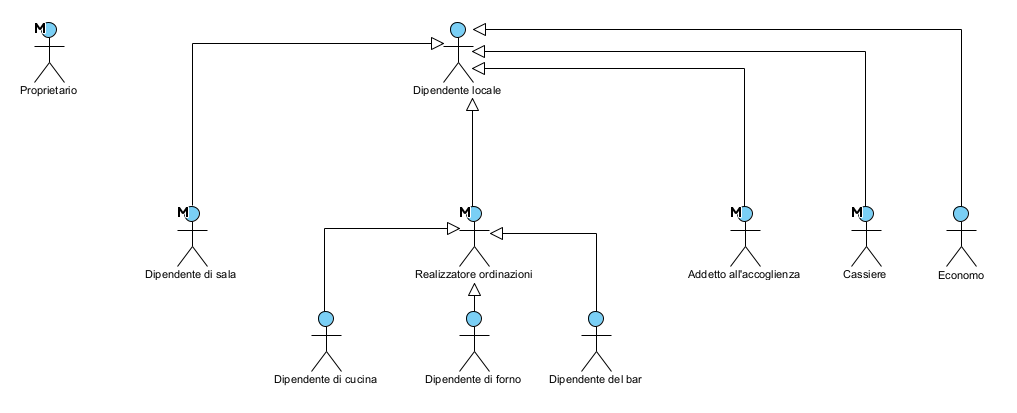
\includegraphics[width=\textwidth]{Immagini/AttoriPrimari.png}
\end{figure}

\begin{itemize}
	\item Dipendente di sala: deve interagire con il cliente e prendere le ordinazioni in maniera tale che vengano smistate, tramite il sistema alle varie attività del locale;
	\item Dipendenti di cucina/forno/bar: usano il sistema per ricevere i vari ordini e per notificare un completamento di essi;
	\item Addetto all'accoglienza: usa il sistema per visualizzare i tavoli disponibili ed assegnarli ai clienti;
	\item Cassiere: richiede al sistema il conto totale di un cliente interessato per completare il pagamento;
	\item Economo: si occupa della gestione delle merci ovvero l'aggiornamento delle quantità presenti in magazzino (in base alle vendite effettuate dalla sala e dalle richieste dei realizzatori di ordinazioni);
	\item Proprietario: può usare il sistema per aggiungere e rimuovere dipendenti, consultare dati come vendite, guadagni, quantità di merci.
\end{itemize}
Nella realtà non tutti gli attori descritti corrisponderanno a persone fisiche differenti, infatti alcuni dipendenti potranno assumere le funzionalità di più attori (ad esempio un dipendente di sala potrebbe ricoprire anche il ruolo di addetto all'accoglienza). A tal proposito quindi si è scelto di intendere gli attori come \textbf{ruoli} che un dipendente reale possa ricoprire.

\section{Attori Finali}
\begin{figure}[H]
	\centering
	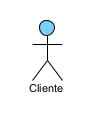
\includegraphics[width=0.12\textwidth]{Immagini/AttoriFinali.png}
\end{figure}

\begin{itemize}
	\item Cliente: pur non interagendo con il sistema, è direttamente interessato in alcuni suoi casi d'uso in quanto gli consentono di usufruire del servizio del locale
\end{itemize}
\newpage

\section{Tabella Attori-Obiettivi}
Dopo aver identificato a pieno gli attori che utilizzeranno il sistema, bisogna associare ad ogni attore i suoi obiettivi.
\begin{table}[!h]
	\centering
	\begin{tabular}{|p{0.3\linewidth}|p{0.65\linewidth}|}
		\hline
		\rowcolor{Red}
		Attore & Obiettivi \\
		\hline
		\hline
		\multirow{9}{6em} {Proprietario} & Inserimento di un dipendente \\
		& Rimozione di un dipendente \\ & Modifica dei ruolo di un dipendente \\
		& Visualizzazione dei dipendenti \\
		& Inserimento di un tavolo\\
		& Rimozione di un tavolo\\
		& Modifica di un tavolo\\
		& Visualizzazione dei tavoli \\
		& Inserimento di prodotti nel menu \\
		& Rimozioni di prodotti dal menu \\
		& Modifica di prodotti del menu \\
		& Visualizzazione del menu completo \\
		
		\hline
		\multirow{4}{6em} {Dipendente di sala} 
		& Creazione di un'ordinazione per un cliente  \\
		& Rimozione di un'ordinazione \\ 
		& Modifica di un'ordinazione \\
		& Visualizzazione delle ordinazioni \\
		\hline
	
		\multirow{3}{6em} {Accoglienza} 
		& Assegnazione di un tavolo a dei clienti  \\
		& Modifica dello stato di un tavolo (libero, occupato, riservato, ecc.) \\ 
		& Visualizzazione di tutti i tavoli \\
		\hline	
		
		\multirow{1}{6em} {Cassiere} 
		& Generazione vendita di un tavolo (pagamento dei clienti)\\ 
		\hline
		
		\multirow{2}{7em} {Realizzatore di ordinazione} 
		& Visualizzazione degli ordini per area (cucina, bar, forno)  \\
		& Notifica completamento ordinazione \\ 
		\hline
		
		\multirow{4}{6em} {Economo} 
		& Inserimento di una merce  \\
		& Modifica di una merce \\ 
		& Rimozione di una merce \\
		& Visualizzazione di una merce \\
		\hline
	\end{tabular}
\end{table}
\\Gran parte degli obiettivi riguardano operazioni \textit{CRUD} (Create, Read, Update, Delete) che possono essere raggruppate in un solo obiettivo.

\newpage
\section{Diagramma dei Casi D'Uso}
Tutti gli obbiettivi CRUD dei vari attori sono stati inglobati in un unico caso d'uso con il prefisso \textbf{Gestisci}, per indicare le operazioni che racchiudono.
\\
\\
\begin{centering}  
	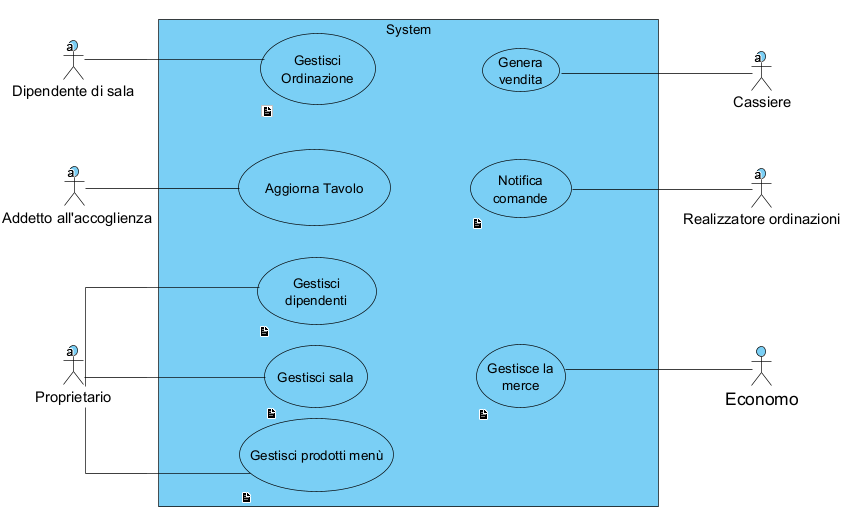
\includegraphics[width=\textwidth]{Immagini/DiagrammaCasiUso.png}
\end{centering}

\subsection{Descrizione Breve}
\subsubsection{Gestisci Ordinazione}
Come descritto in precedenza questo caso d'uso racchiude le operazioni CRUD riguardo ad un'ordinazione di uno o più clienti. Il cameriere infatti deve essere in grado di creare un'ordinazione per un cliente e poterla in seguito modificare, visualizzare o addirittura rimuovere dal sistema.

\subsubsection{Aggiorna Tavolo}
L'addetto all'accoglienza si occupa di far accomodare i clienti nella sala. Il suo obiettivo è quindi avere una visione completa dei tavoli comunicando tramite il sistema  quali tavoli hanno clienti in attesa di ordinazione, quali sono liberi e quali sono occupati.

\subsubsection{Gestisci Dipendenti}
Il proprietario può aggiungere/rimuovere dipendenti dal sistema ed inoltre è in grado di decidere/modificare i ruoli o il ruolo di ogni dipendente durante il servizio.

\subsubsection{Gestisci Sala}
Il proprietario può indicare l'identificativo di ogni tavolo in relazione alla sala in cui appartiene. Gli altri dipendenti quindi posso accedere tramite l'identificativo a tutte le informazioni che riguardano i tavoli (numero di persone accomodate, lista dei prodotti ordinati, ecc).

\subsubsection{Gestisci Prodotti Menù}
Il proprietario può effettuare operazioni CRUD per la gestione del menù del locale.

\subsubsection{Genera Vendita}
Il compito del cassiere è quello di registrare il pagamento dei clienti in relazione a ciò che hanno ordinato. Esso quindi deve poter risalire tramite il tavolo a tutti gli ordini associati ai clienti per ricavare il prezzo complessivo da pagare.

\subsubsection{Notifica Ordinazione}
Per rendere il sistema quanto più automatizzato possibile, i realizzatori di ordinazioni (cuoco, pizzaiolo, etc.) devono notificare il completamento di un'ordinazione tramite il sistema. In questo modo, inviando una notifica il sistema provvederà ad avvisare altri dipendenti in attesa di quel completamento.

\subsubsection{Gestisci Merce}
Ogni prodotto del menu è composto da un insieme di merci disponibili in magazzino. Il compito dell'economo è quindi quello di gestire le merci, per avere sotto controllo le merci in esaurimento. L'esaurimento di una merce comporta la non disponibilità di tutti i prodotti del menu che la contenevano.

\subsection{Descrizione Dettagliata}
La descrizione dettagliata è stata fatta solo per i casi d'uso di rilievo.
\begin{longtable}[htbp]{|p{0.3\linewidth}|p{0.65\linewidth}|}
	\hline
		\rowcolor{Blue}	
	\textbf{Titolo} & Gestisci Ordinazione \\[0.3cm]
	\hline
	\textbf{Livello} & Obiettivo Utente \\[0.3cm]
	\hline
	\textbf{Portata} & Applicazione Android/Desktop Lightning Order\\[0.3cm]
	\hline
	\textbf{Attore Primario} & Dipendente di sala \\[0.3cm]
	\hline
	\multirow{6}*{\textbf{Parti Interessate}} 
	& \textendash \underline{Dipendenti di sala} (vogliono registrare/modificare un'ordinazione) \\
	& \textendash \underline{Proprietario} (vuole che i clienti siano serviti) \\
	& \textendash \underline{Clienti} (vogliono ricevere quanto ordinato) \\
	& \textendash \underline{Realizzatore di ordinazioni} (vuole essere aggiornato sulle ordinazioni) \\[0.3cm]
	\hline
	\multirow{5}*{\textbf{Pre-Condizioni}}
	& \textendash Il dipendente di sala è autenticato e ha il ruolo di cameriere \\
	& \textendash Il tavolo che sta prendendo l'ordinazione non è nello stato di libero\\[0.3cm]
	\hline

	\multirow{5}*{\textbf{Garanzia di successo}}
	& \textendash Un'ordinazione viene creata/modificata/rimossa \\
	& \textendash Una notifica viene inviata ad un realizzatore di ordinazione \\
	& \textendash La merce numerabile costituente i prodotti viene riservata o ripristinata in caso di eliminazione/modifica\\[0.3cm]
	\hline
	\multirow{8}*{\textbf{Scenario Principale}} 
	& 1. Dipendente di sala richiede di visualizzare la lista dei tavoli \\
	& 2. Il sistema mostra i tavoli in attesa\\
	& 3. Dipendente di sala seleziona un tavolo \\
	& 4. Il sistema mostra la lista di ordinazioni del relativo tavolo \\
	& 5. Il cliente richiede un'operazione (crea/modifica/elimina ordinazione)\\
	& 6. Il sistema riceve la modifica e notifica gli interessati.\\[0.3cm]
	\hline
	
	\newpage
	\multirow{28}*{\textbf{Estensioni}}
	& 5.A Dipendente di sala seleziona ordinazione a tavolo \\
	& 6.A Cliente comunica i prodotti \\
	& 7.A Il dipendente di sala inserisce prodotti con eventuali merci aggiuntive \\
	& 8.A Il cliente comunica preferenza di consegna per prodotti \\
	& 9.A Il dipendente di sala inserisce la preferenza di consegna \\
	& 10.A Il dipendente di sala aggiunge ordinazione \\
	& 11.A Il sistema riceve la modifica \\
	& 12.A Vengono inviate notifiche ai realizzatori di ordinazioni \\
	& \\
	
	& 5.B Il dipendente di sala rimuove l'ordinazione selezionata \\
	& 6.B Il sistema riceve la modifica\\
	& 7.B Il sistema notifica l’evento ad eventuali realizzatori \\
	
	
	& \\
	& 5.D Cliente comunica al dipendente di aggiungere un prodotto all'interno di un'ordinazione \\
	& 6.D Dipendente aggiunge il prodotto (o i prodotti) all'ordinazione \\
	& 7.D Il sistema viene aggiornato e invia una notifica ai realizzatori \\[0.3cm]
	
	& \\
	& 5.E Cliente comunica al dipendente di rimuovere un prodotto all'interno di un'ordinazione \\
	& 6.E Dipendente rimuove il prodotto (o i prodotti) all'ordinazione \\
	& 7.E Il sistema viene aggiornato e invia una notifica ai realizzatori \\[0.3cm]
	

	\hline
	\multirow{10}*{\textbf{Scenari Alternativi}}
	& 11.A.1 L'ordinazione registrata è la prima per quel tavolo\\
	& 11.A.2 Il sistema cambia lo stato del tavolo da \textit{"in attesa di ordinazione"} in \textit{"occupato"}\\
	&\\
	& 5.A.1 Prodotto comunicato non è disponibile \\
	& 5.A.2 Ripeti 5 \\
	& \\
	& 5.C.1 L'ordinazione non è modificabile (poiché in lavorazione) \\
	& 5.C.2 Ripeti 5\\
	& \\
	& 5.D.1 Il prodotto non è disponibile \\
	& 5.D.2 Ripeti 5 \\
	& \\
	& 5.E.1 Il prodotto non è rimovibile (poiché in lavorazione) \\
	& 5.E.2 Ripeti 5\\[0.3cm]
	\hline
\end{longtable}

\vspace*{1.5 cm}


\begin{longtable}[htbp]{|p{0.3\linewidth}|p{0.65\linewidth}|}
	\hline
	\rowcolor{LightCyan}
	\textbf{Titolo} & Aggiorna Tavolo\\[0.3cm]
	\hline
	\textbf{Livello} & Obiettivo Utente \\[0.3cm]
	\hline
	\textbf{Portata} & Applicazione Android/Desktop Lightning Order\\[0.3cm]
	\hline
	\textbf{Attore Primario} & Addetto all'accoglienza\\[0.3cm]
	\hline
	\multirow{6}*{\textbf{Parti Interessate}} 
	& \textendash \underline{Dipendenti di sala} (vogliono avere una visione aggiornata dello stato dei tavoli) \\
	& \textendash \underline{Cliente} (vuole accomodarsi) \\
	& \textendash \underline{Proprietario} (vuole che i clienti entrino ed escano in maniera ordinata) \\[0.3cm]
	\hline
	\multirow{2}*{\textbf{Pre-Condizioni}}
	& \textendash Il dipendente ha effettuato il login e ricopre il ruolo di addetto all'accoglienza\\[0.3cm]
	\hline
	\multirow{6}*{\textbf{Garanzia di successo}}
	& \textendash Il cliente occupa il tavolo \\
	& \textendash Lo stato del tavolo viene aggiornato\\
	& \textendash I camerieri ricevono la notifica di un nuovo tavolo da servire\\[0.3cm]
	\hline
	\newpage
	\multirow{7}*{\textbf{Scenario Principale}} 
	& 1. Addetto all'accoglienza richiede di visualizzare i tavoli di una sala\\
	& 2. Il sistema mostra i tavoli con il relativo stato\\
	& 3. L'addetto all'accoglienza seleziona un tavolo per cui aggiornare lo stato\\
	& 4. Il sistema registra la modifica e notifica i camerieri in caso di tavolo appena occupato\\[0.3cm]
	\hline
	\multirow{5}*{\textbf{Estensioni}}
	& 3.A L'addetto all'accoglienza seleziona un tavolo nello stato \textit{"occupato"}\\
	& 4.A L'addetto all'accoglienza seleziona l'aggiornamento dello stato del tavolo in \textit{"libero"}\\
	&\\
	& 3.B L'addetto all'accoglienza seleziona un tavolo \textit{libero}\\
	& 4.B L'addetto all'accoglienza seleziona l'aggiornamento dello stato del tavolo in \textit{"in attesa di ordinazione"}\\[0.3cm]
	\hline
\end{longtable}

\vspace*{1.0 cm}

\begin{longtable}[htbp]{|p{0.3\linewidth}|p{0.65\linewidth}|}
	\hline
	\rowcolor{Green}
	\textbf{Titolo} & Notifica Ordinazione \\[0.3cm]
	\hline
	\textbf{Livello} & Obiettivo Utente \\[0.3cm]
	\hline
	\textbf{Portata} & Applicazione Android/Desktop Lightning Order\\[0.3cm]
	\hline
	\textbf{Attore Primario} & Realizzatore di ordinazione \\[0.3cm]
	\hline
	\multirow{6}*{\textbf{Parti Interessate}} 
	& \textendash \underline{Realizzatore di ordinazione} (vuole notificare ad altri realizzatori e ai camerieri l’aver completato uno o più lavori). \\
	& \textendash \underline{Cliente} (vuole ricevere l’ordinazione). \\
	& \textendash \underline{Proprietario} (vuole che cliente riceva l’ordinazione) \\[0.3cm]
	\hline
	\multirow{1}*{\textbf{Pre-Condizioni}}
	& \textendash L'ordinazione da segnare come completata è registrata nel sistema\\[0.3cm]
	\hline
	\newpage
	\multirow{6}*{\textbf{Garanzia di successo}}
	& \textendash Prodotto in ordinazione viene posto in stato di terminato \\
	& \textendash Qualora i prodotti di tutta l’ordinazione vengano posti come terminati allora anche l’ordinazione stessa viene posta come terminata \\[0.3cm]
	\hline
	\multirow{7}*{\textbf{Scenario Principale}} 
	& 1. Realizzatore richiede ordinazioni al sistema \\
	& 2. Il sistema restituisce le ordinazioni che può eseguire \\
	& 3 Il realizzatore seleziona un prodotto \\
	& 4 Il sistema restituisce i dati del prodotto \\
	& 5. Il realizzatore notifica il completamento del prodotto \\
	& 6. Il sistema si aggiorna \\
	& 7. Il sistema sblocca prodotti pendenti \\[0.3cm]
	\hline
	\multirow{5}*{\textbf{Estensioni}}
	& 5.A Il prodotto completato era l'ultimo \\
	& 6.A Il sistema aggiorna lo stato dell'ordinazione \\
	& 7.A Il sistema invia un'ordinazione pendente per altri realizzatori di ordinazione in attesa di quel completamento	\\[0.3cm]
	\hline
	\multirow{1}*{\textbf{Scenari Alternativi}}
	& 7.B.1 Non ci sono ordini pendenti \\[0.3cm]
	\hline
\end{longtable}
\newpage
\section{Requisiti non funzionali}
Il sistema oltre a realizzare i requisiti descritti precedentemente deve rispettare dei vincoli di funzionamento. Tutti i requisiti non funzionali vengono descritti tramite delle specifiche supplementari di tipo \textbf{FURPS+}

\subsection{Funzionalità}
Per tutti i casi d'uso deve esistere una gestione degli errori ottimale. Durante il funzionamento dell'applicazione, il sistema non deve interrompersi a causa degli errori non gestiti.

\subsection{Usabilità}
L'interfaccia utente deve essere semplice e intuitiva permettendo così al dipendente di interagire con il sistema nel modo più veloce possibile.
\\Per quanto riguarda i camerieri, l'applicativo può essere installato sul proprio dispositivo mobile (ad esempio il proprio smartphone) in modo tale da ridurre al minimo i costi per dispositivi dedicati.
Per i dipendenti i quali dispongono di una postazione fissa l'applicativo sarà invece in esecuzione su un computer fisso con monitor touch screen in modo da rendere l'interazione con l'applicazone semplice e veloce.

\subsection{Affidabilità}
Il sistema deve garantire un corretto coordinamento tra i dipendenti della sala e una prevenzione degli errori impedendo ad esempio che : 
\begin{itemize}
	\item una stessa ordinazione venga presa in carico da due realizzatori contemporaneamente;
	\item un articolo terminato (unità finite nel caso di una bevanda o per assenza di materie prime nel caso di una pietanza) possa essere ordinato da un cliente.
\end{itemize}
Ogni ordine registrato deve poter essere modificato, in particolare deve essere possibile eliminare uno degli articoli che ne fanno parte o l'intero ordine. 
Inoltre il proprietario deve avere la possibilità di gestire tutti gli utenti iscritti all'applicazione. In altre parole nel momento in cui un dipendente non farà più parte dell'azienda questo deve poter essere eliminato dalla \textit{user list} in modo da impedirgli l'accesso all'applicazione con le sue vecchie credenziali.
%aggiungere NO modifica proprie credenziali

\subsection{Prestazioni}
Il sistema deve funzionare in tempo reale. La gestione delle ordinazioni, soprattutto, deve poter rispondere immediatamente a variazioni, modifiche e aggiunte di eventuali ordinazioni nel sistema, per notificare velocemente coloro che dovranno realizzarle ed evitare così possibili incomprensioni tra reparti.

\subsection{Sostenibilità}
Nel lato "mobile" il sistema deve adattarsi alla maggior parte degli smartphone in commercio, onde evitare problemi di compatibilità. \\
Nel lato "desktop" il sistema deve essere portabile per poter essere configurato in un qualunque ambiente. 




